Dieser Abschnitt widmet sich den Funktionalitäten, die sich in der dll baseqt.dll befinden. Eine Funktionalität wurde bereits im Kapitel Konfiguration vorgestellt: Alle Klassen für das Arbeiten mit Konfigurationen befinden sich auch in baseqt.dll.\bigskip \\
\textbf{AboutDialog}\\
Die Klasse AboutDialog stellt einen Informationsdialog über die Anwendung selber bereit, siehe Abbildung \ref{fig:AboutDialog}. Die Methoden der Klasse sind:
\begin{description}
	\item[ ] explicit AboutDialog(QString programName, QString programVersion, QWidget *parent $=$ 0)\\
	Konstruiert ein neues Objekt von AboutDialog. Dabei müssen der Programmname (programName), die Version des Programms (programVersion) und, wie für Qt üblich, ein parent (dieser kann auch weggelassen werden, ist aber nicht ratsam) übergeben werden.
   \item[ ] \~{}AboutDialog()\\
	Zerstört das Objekt wieder und gibt den Speicherplatz frei.
\end{description}
\begin{figure}[htb]
	\centering
		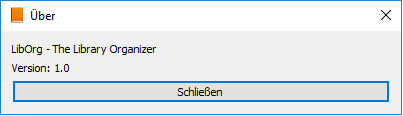
\includegraphics[width=0.60\textwidth]{figures/AboutDialog.png}
	\caption{AboutDialog}
	\label{fig:AboutDialog}
\end{figure}

\textbf{BaseException}\\
Die Klasse BaseException stellt eine Fehlerklasse dar. Im Gegensatz zur Qt-Variante für Exceptions (QException) wird der Fehlertext im Abbruchsfenster gezeigt.\\
Die Basisklasse von BaseException ist std::exception.\\
Die Klasse enthält folgende Methoden und öffentliche Member:
\begin{description}
	\item[ ] enum ErrorCode: ErrorInCode (100)\\
	Beschreibt den aufgetretenen Fehler in Form eines Codes. Derzeit existieren nur Fehler, die auf Fehler im Quellcode, also die Programmierung, zurückzuführen sind.
  \item[ ] BaseException(ErrorCode code, QString explanation)\\
	Erstellt ein neues BaseException-Fehlerobjekt unter Angabe des Fehlercodes (code) und einer Beschreibung (explanation).
  \item[ ] \~{}BaseException()\\
	Zerstört das Objekt und gibt den Speicherplatz frei.
  \item[ ] const char* what() const noexcept\\
	Diese Methode liefert den Fehlertext des Fehlerobjektes zurück. 
\end{description}

\textbf{ConfigDialog}\\
Die Klasse ConfigDialog dient als Basisklasse für beliebige Dialoge, die mit den Konfigurationsklassen einen Einstellungsdialog bilden können. Die Methoden der Klasse sind:
\begin{description}
	\item[ ] virtual void setModified(bool modified) = 0\\
	Diese virtuelle Methode hat in der Klasse keine Implementierung. Sie muss in der abgeleiteten Klasse implementiert werden und dient dazu, zu markieren, dass sich Werte von Konfigurationen innerhalb des Dialogs geändert haben.
\end{description}

\textbf{ConfigWidget}\\
ConfigWidget stellt ein Widget zur Anzeige und Bearbeitung aller Konfigurationseinträge bereit. Alle Elemente eines Konfigurationsblockes können ein- und ausgeblendet werden.\\
Die Basisklassen sind: QWidget und ConfigObserver.\\
Methoden:
\begin{description}
	\item[ ] explicit ConfigWidget(Config* cfg, ConfigDialog *parentDialog, QWidget *parent = nullptr)\\
	Erzeugt ein neues ConfigWidget. Dabei wird für jeden Eintrag in Config ein entsprechendes Darstellungswidget (configwidgetelement) erstellt. Der Klasse muss der parentDialog sowei ein parent übergeben werden.
  \item[ ] \~{}ConfigWidget()\\
		Zerstört das Widget mit allen untergeorndeten child-Widgets.
  \item[ ] void cfgblockchanged(QString blockname, Action action) noexcept\\
		Mit der Methode wird dem ConfigDialog mitgeteilt, dass sich der Blockname entsprechend der action geändert hat.
  \item[ ] void cfgkeyofblockchanged(QString blockname, QString keyname, Action action) noexcept\\
	Diese Methode dient dazu dem ConfigDialog mitzuteilen, sich sich der Konfigruationseintrag gemäß blockname und keyname entsprechend der action geändert hat.
\end{description}

\textbf{ConfigWidgetElement}\\
Ein ConfigWidgetElement stellt basierend auf dem Konfigurationsschlüssel ein passendes Widget bereit. Die Basisklasse ist QWidget. Die Klasse enthält folgende Methoden:
\begin{description}
	\item[ ] explicit ConfigWidgetElement(QString blockname, QString keyname, Config* cfg, QWidget *parent = nullptr)\\
	Erzeugt basierend auf dem Konfigurationsschlüssel blockname und keyname aus der Config ein entsprechendes Anzeigeelement. Wie üblich, sollte ein parent-Objekt übergeben werden.
   \item[ ] \~{}ConfigWidgetElement()\\
	  Zerstört das Anzeigeelement wieder.
\end{description}

\textbf{SettingsDialog}\\
Die Klasse SettingsDialog stellt einen Dialog zur Anzeige und Bearbeitung von Konfigurationsdateien, siehe Abbildung \ref{fig:SettingsDialog}, dar. Die Klasse ist abgeleitet von QDialog und ConfigDialog. Ihre Methoden sind:
\begin{description}
	\item[ ] explicit SettingsDialog(Config *cfg, QWidget *parent = 0)\\
	Erzeugt einen neuen Dialog unter Übergabe einer Konfigurations (cfg) und eines parents. Der Dialog enthält beim Anzeigen für jeden Konfigurationsschlüssel ein eigenes Widget zu dessen Bearbeitung und Anzeige. Jeder Konfigurationsblock kann eingeklappt werden.
	\item[ ] \~{}SettingsDialog()\\
	Zerstört das Objekt und löscht alle Kindelemente.
	\item[ ] void setModified(bool modified)\\
	Diese Methode musste von ConfigDialog überladen und implementiert werden. Ändert sich ein Konfigurationseintrag, so wird dies am Dialogstitel durch ein * gekennzeichnet. Wird der Dialog nun geschlossen, so wird vorab nachgefragt, ob die Änderungen gespeichert werden sollen.
\end{description}
\begin{figure}[htb]
	\centering
		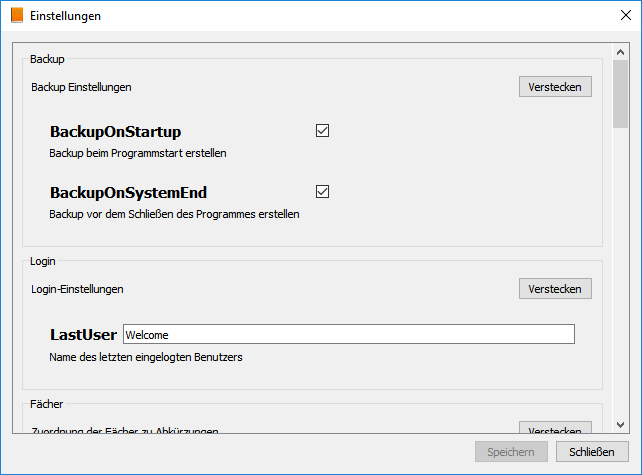
\includegraphics[width=0.70\textwidth]{figures/SettingsDialog.png}
	\caption{SettingsDialog (Beispiel)}
	\label{fig:SettingsDialog}
\end{figure}

\textbf{Licenceplugin}\\
Die Klasse Licenceplugin stellt einen Plugin-Mechanismus zur Anzeige von Lizenztexten bereit. Licenceplugin ist von QObject abgeleitet und besitzt folgende Methoden:
\begin{description}
	\item[ ] static void CreatePlugin()\\
	Erzeugt das Plugin.
  \item[ ] static void DeletePlugin()\\
	Das Plugin wird zerstört.
  \item[ ] static void Add3rdPartyLicence(LicenceItem *item)\\
	Diese Methode hängt eine neue Lizenz (LicenceItem) an das Plugin an.
  \item[ ] static Licenceplugin* Instance()\\
	Liefert die Instanz des Plugins zurück.
  \item[ ] static void ShowLicences(QWidget *parent)\\
	Erzeugt einen Dialog, der alle Lizenzen anzeigt. Dieser Methode wird der parent für den Dialog übergeben.
\end{description}
Licenceplugin ist unter Verwendung des Singelton Patterns implementiert worden, allerdings nicht threadsafe. Aus diesem Grund kann ein Objekt dieser Klasse nur durch die statische Methode CreatePlugin() erzeugt werden.

\textbf{LicenceItem}\\
Die Klasse LicenceItem stellt eine Basisklasse für Lizenzdateien bereit, die in das Licenceplugin eingefügt werden können. Das LicenceItem ist von QObject abgeleitet. Seine Methoden sind:
\begin{description}
	\item[ ] LicenceItem()\\
	Erzeugt ein neues LicenceItem.
  \item[ ] virtual \~{}LicenceItem()\\
	Zerstört das LicenceItem.
  \item[ ] virtual QPushButton* getButton(QWidget* parent)\\
	Erzeugt einen neuen Button für das LicenceItem und gibt diesen zurück. Der parent des Buttons wird auf parent gesetzt.
  \item[ ] virtual QPushButton* getButton()\\
	Liefert den erzeugten Button für das LicenceItem zurück, erstellt einen Button, falls noch keiner erstellt worden ist.
  \item[ ] virtual QWidget* getWidget(QWidget* parent)\\
	Erstellt ein Widget für das LicenceItem und gibt dieses zurück. Das Widget erhält als parent parent.
  \item[ ] virtual QWidget* getWidget()\\
	Liefert das Widget für das LicenceItem zurück, ggf. wird ein neues Widget ohne parent erzeugt.
  \item[ ] virtual void removeWidget()\\
	Zerstört das Widget des LicenceItem und gibt dessen Speicherplatz frei.
\end{description}

